\documentclass[PhysicsII/physicsII_notes.tex]{subfiles}
\begin{document}
\section{Aula 23 - 18/10/2023}
\subsection{Motivações}
\begin{itemize}
	\item Ondas Estacionárias;
	\item Ondas em Tubos;
	\item Início de Efeito Doppler.
\end{itemize}
\subsection{Ondas Estacionárias}
Considere uma corda presa entre duas superfícies que começa a vibrar. Dependendo da velocidade que ela vibra,
o comprimento de onda \(\lambda \) irá mudar, assim como a frequência
\begin{center}
	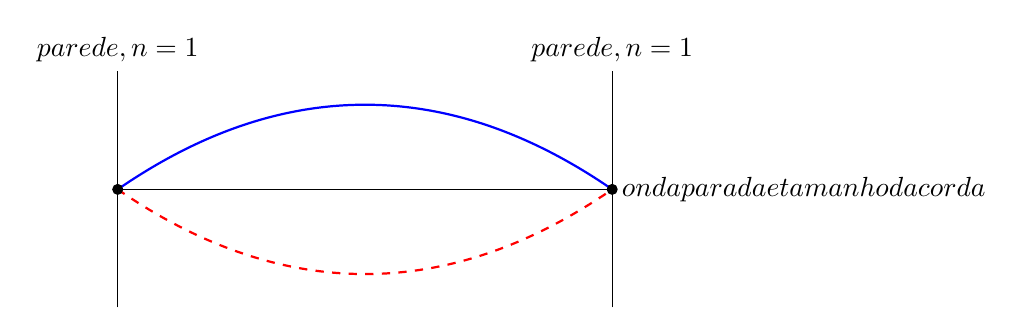
\begin{tikzpicture}
		% Eixos
		\draw[-] (0,0) -- (6.28,0) node[right] {\(\text{onda parada e tamanho da corda}\)};
		\draw[-] (0,-1.5) -- (0,1.5) node[above] {\(\text{parede, n=1}\)};
		\draw[-] (6.28,-1.5) -- (6.28,1.5) node[above] {\(\text{parede, n=1}\)};

		% Onda estacionária sólida
		\draw[thick,blue] plot[domain=0:6.28,samples=200] (\x,{6.28*sin(\x*6.28 - \x*\x)});

		% Onda estacionária tracejada com fase oposta
		\draw[thick,dashed,red] plot[domain=0:6.28,samples=200] (\x,{-6.28*sin(\x*6.28 - \x*\x)});

		% Nós
		\foreach \x in {0, 6.28} {
				\fill (\x,0) circle (2pt);
			}
	\end{tikzpicture}

	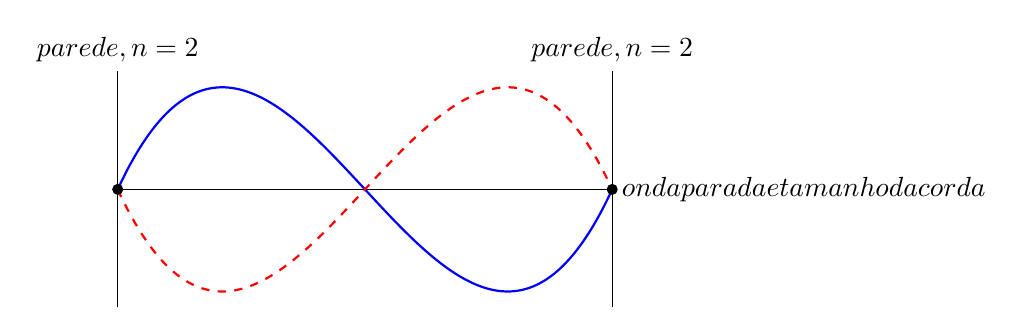
\begin{tikzpicture}
		% Eixos
		\draw[-] (0,0) -- (6.28,0) node[right] {\(\text{onda parada e tamanho da corda}\)};
		\draw[-] (0,-1.5) -- (0,1.5) node[above] {\(\text{parede, n=2}\)};
		\draw[-] (6.28,-1.5) -- (6.28,1.5) node[above] {\(\text{parede, n=2}\)};

		% Onda estacionária sólida
		\draw[thick,blue] plot[domain=0:6.28,samples=200] (\x,{6.28*sin((3.14-\x)*(\x*6.28 - \x*\x))});

		% Onda estacionária tracejada com fase oposta
		\draw[thick,dashed,red] plot[domain=0:6.28,samples=200] (\x,{-6.28*sin((3.14-\x)*(\x*6.28 - \x*\x))});

		% Nós
		\foreach \x in {0, 6.28} {
				\fill (\x,0) circle (2pt);
			}
	\end{tikzpicture}

	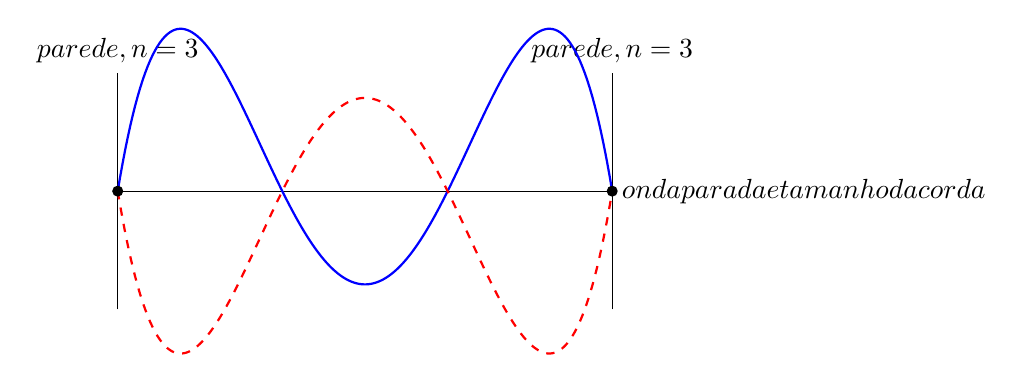
\begin{tikzpicture}
		% Eixos
		\draw[-] (0,0) -- (6.28,0) node[right] {\(\text{onda parada e tamanho da corda}\)};
		\draw[-] (0,-1.5) -- (0,1.5) node[above] {\(\text{parede, n=3}\)};
		\draw[-] (6.28,-1.5) -- (6.28,1.5) node[above] {\(\text{parede, n=3}\)};

		% Onda estacionária sólida
		\draw[thick,blue] plot[domain=0:6.28,samples=200] (\x,{6.28*sin((4.19-\x)*(2.09-\x)*(\x*6.28 - \x*\x))});

		% Onda estacionária tracejada com fase oposta
		\draw[thick,dashed,red] plot[domain=0:6.28,samples=200] (\x,{-6.28*sin((4.19-\x)*(2.09-\x)*(\x*6.28 - \x*\x))});

		% Nós
		\foreach \x in {0, 6.28} {
				\fill (\x,0) circle (2pt);
			}
	\end{tikzpicture}
\end{center}
(Os picos deveriam estar do mesmo tamanho!!!!)
Obtemos a seguinte tabela representando as mudanças
\begin{center}
	\begin{table}[h!]
		\caption{Quantidades de Acordo com a Velocidade}
		\centering
		\begin{tabular}{| c | c | c |}
			\hline
			n & \(\lambda \)     & f                 \\
			\hline
			1 & 2L               & \(\frac{2v}{2L}\) \\
			2 & \(\frac{2L}{2}\) & \(\frac{2v}{2L}\) \\
			3 & \(\frac{2L}{3}\) & \(\frac{3v}{2L}\) \\
			4 & \(\frac{2L}{4}\) & \(\frac{4v}{2L}\) \\
			\hline
		\end{tabular}
	\end{table}
\end{center}
Observando esta tabela, chamamos o caso n=1 de primeiro harmônico fundamental, n=2 de segundo harmônico fundamental, e assim em diante. Além disso, há a seguinte relação:
\[
	\lambda = \frac{2L}{n},\quad f = n \frac{v}{2L},\quad \lambda = \frac{\lambda_{1}}{n},
\]
em que n é um natural, \(v = \sqrt[]{\frac{F_{T}}{\mu}}\) e \(\lambda_{1}\) é o comprimento de onda no primeiro harmônico fundamental. Em particular, segue que
\[
	f = n f_{1},\quad n\in \mathbb{N}.
\]
\begin{example}
	Considere uma corda vibrando em \(f = 440Hz\) de tamanho \(L - 0.7m\). Neste caso, temos
	\[
		\lambda  = 2L = 1.4m,\quad v = f\lambda = 440\times 1.4 = 616\frac{m}{s}.
	\]
\end{example}
\begin{example}
	Considere uma corda de piano de 3m com densidade linear de massa \(\mu = 0.0025 \frac{kg}{m}\) e suponha que ela vibra em duas frequências - \(f_{n} = 252Hz\) e \(f_{n+1} = 336Hz\)
	(não sabemos qual nó que é). A tensão máxima que a corda pode ser submetida é \(F_{max} = 700N.\) Esta corda está a ponto de estourar?

	Sabemos que \(v^{2} = \frac{F_{T}}{\mu}\) e que \(v = \frac{f}{n}2L\). Assim,
	\[
		F_{T} = \mu \biggl[\frac{f_{n}2L}{n}\biggr]^{2}.
	\]
	Como \(f_{n} = nf_{1}\) e \(f_{n+1} = (n+1)f_{1}\), temos
	\[
		\frac{f_{n}}{f_{n+1}} = \frac{n}{n+1} \Rightarrow \frac{252}{336} = \frac{n}{n+1},
	\]
	tal que
	\[
		336n = 252n + 252 \Rightarrow 84n = 252 \Rightarrow n = \frac{252}{84} = 3.
	\]
	Em outras palavras, o terceiro harmônico fundamental é o que vale 252, o que permite-nos simplificar
	\[
		F_{T} = \mu \biggl[\frac{nf_{1}2L}{n}\biggr]^{2} = \mu f_{1}^{2}4L^{2} = \mu \biggl(\frac{f_{3}}{3}\biggr)^{2}4L^{2} = \mu 84^{2}4L^{2} = 635N.
	\]
	Portanto, a corda não está prestes a estourar.
\end{example}
Se a corda não estiver presa a um ponto, os harmônicos ocorrem apenas para n's ímpares, tal que
\[
	\lambda_{n} = \frac{4L}{n} = \frac{\lambda_{1}}{n},\quad f_{n} = \frac{nv}{4L} = nf_{1},\quad n = 1, 3, 5, \cdots
\]

Agora, considere \(y = A(x)\cos^{}{(\omega t + \delta )}\). Se \(\cos^{}{(\omega t + \delta )}=1,\) segue que
\[
	A_{0}\sin^{}{(k_{n}x)} = A(x),\quad k_{n} = \frac{2\pi }{\lambda_{n}}.
\]
Se supormos que \(A(0) = 0 = A(L)\), então \(\frac{2\pi }{\lambda_{n}}\) é um número inteiro múltiplo de L, donde obtemos
\[
	\frac{2\pi }{n}L = n\pi \Rightarrow \lambda_{n} = \frac{2L}{n},
\]
já que seno anula-se nos valores múltiplos de \(\pi \). Com isso,
\[
	y(x, t) = A\sin^{}{(k_{n}x)}\cos^{}{(\omega t + \delta )}.
\]
\subsection{Ondas Sonoras em Tubos}
A teoria construída até agora será usada para descrever ondas sonoras em tubos abertos e em tubos fechados, pois ela depende fortemente
da questão dos harmônicos. Um disclaimer importante de ser feito é que, dependendo do material base, o desenho mudará - alguns livros representam
o deslocamento das partículas, outros representam a pressão.

Primeiramente, considere um tubo aberto. Em suas extremidades, devem haver nós, pois a pressão deve ser a mesma que o exterior. Conforme avança-se
em direção ao centro, essa pressão aumenta. No ponto de vista do deslocamento, há mais dele nas extremidades e vai reduzindo conforme avança-se para o
centro. Voltamos ao caso da corda presa em duas posições

Quanto ao tubo fechado, ao chegar à extremidade sem saída, o deslocamento será na menor quantidade, mas a pressão estará em um máximo.
Em contraste com o primeiro, este é o caso da corda presa em uma posição só.
\begin{example}
	Considere um órgão (instrumento) e seu tubo aberto, com comprimento L de 1m. Qual é a frequência do modo fundamental?

	Temos \(\lambda  = 2L = 2m. \) Como a velocidade do som é \(343 \frac{m}{s}\), segue que
	\[
		v = \lambda f \Rightarrow f = \frac{v}{\lambda } = 171.5 Hz
	\]
	Caso fosse hélio ao invés de ar, como a velocidade do hélio é \(v_{He} = 975m/s\),
	\[
		f = \frac{v}{\lambda } \approx 480Hz.
	\]
\end{example}
Preencha um tubo de água e conecte-o a um reservatório por meio de uma mangueira, sendo este reservatório móvel para cima e para baixo. Com um diapasão,
você acerta o tubo com uma frequência conhecida e abaixa o reservatório. Quando a coluna estiver em ressonância com a frequência, um som mais alto é produzido.
Em outras palavras, estamos medindo as ondas do tubo, permitindo-nos medir os comprimentos de ondas nesse tubo de acordo com a altura que a coluna d'água entrou em ressonância.

Certa vez, utilizando um diapasão de 500Hz, foram medindo e mediram os seguintes valores:
\[
	L = 16;\quad50,5;\quad85;\quad119,5cm
\]
tal que \(\Delta L = 119.5 - 85 = \frac{\lambda }{2}\). Sabendo a frequência e o \(\lambda \), descobriram a velocidade do som como \(v\approx 345m/s.\)
\subsection{Efeito Doppler}
Para estudar este efeito, assume-se que a fonte da onda é móvel tal que ela desloca-se \(u_{f}T\). Para um observador olhando, o comprimento da onda de antes dela
mover-se comparado com o comprimento após o movimento será maior no segundo caso. Antes dela mover-se, a velocidade vale \(f_{O}\lambda_{O} = v\).
Sabemos o comprimento de onda como sendo \(\lambda_{0} = (v-u_{f})T\), donde obtemos, para o caso da fonte aproximando-se, a frequência percebida pelo observador
\[
	f_{O} = \frac{v}{(v-u_{f})T} = \frac{vf_{F}}{v-u_{f}} = \frac{f_{f}}{1-\frac{u_{f}}{v}},
\]
em que \(f_{F}\) é a frequência da fonte. Analogamente, caso a fonte esteja afastando-se,
\[
	f_{O} = \frac{f_{F}}{1+\frac{u_{f}}{v}}.
\]
\end{document}
